%!TEX program = xelatex
\PassOptionsToPackage{table,svgnames}{xcolor}
\PassOptionsToPackage{french}{babel}
\PassOptionsToPackage{french}{translator}
%\documentclass[aspectratio=169,11pt]{beamer}
\documentclass[11pt]{beamer}

%----------------------------------------
% Packages
%----------------------------------------

% Pro­gram­ming fa­cil­i­ties
\usepackage{etoolbox}
\usepackage{ifxetex}
\usepackage{ifluatex}

% Encoding
\usepackage[T1]{fontenc}
\ifboolexpr{bool{xetex} or bool{luatex}}{%
	\usepackage{fontspec}
}{%
	\usepackage[utf8]{inputenc}
}

% Language
\usepackage[french]{babel}
\usepackage[french]{translator}

% General purpose
\usepackage{hyperref}
\usepackage{xcolor}
\usepackage{tcolorbox}
\usepackage{pdflscape}
\usepackage{relsize}
\usepackage{fancyvrb}

% Algorithms
\usepackage[linesnumbered,ruled,vlined]{algorithm2e}

% Mathematics
\usepackage{amsmath}
\usepackage{amssymb}
\usepackage{mathrsfs}
\usepackage{amsthm}
\usepackage{dsfont}
\usepackage{braket}
\usepackage{stmaryrd}

% Tables
\usepackage{array}
\usepackage{tabularx}
\usepackage{longtable}
\usepackage{tabu}
\usepackage{booktabs}
\usepackage{multirow}
\usepackage{makecell}
\usepackage{blkarray}

% Figures
\usepackage[mode=tex]{standalone}
\usepackage{import}
\usepackage{float}
\usepackage[justification=centering]{caption}

% PGF-TikZ
\usepackage{pgf}
\usepackage{pgfplots}
\pgfplotsset{compat=1.16}
\usepackage{tikz}
\usepackage{tikzpeople}
\usepackage{pgf-umlsd}
\usepackage{pgfgantt}

% Bibliography
\usepackage[backend=biber,bibstyle=ieee,citestyle=numeric-comp]{biblatex}

%----------------------------------------
% Definitions
%----------------------------------------

%!TEX encoding = UTF-8 Unicode

% C++
\newcommand{\Cpp}{\texorpdfstring{C\kern-0.05em\protect\raisebox{.35ex}{\textsmaller[2]{+\kern-0.05em+}}}{C++}}

% Clear to the next left page
\newcommand*{\cleartoleftpage}{
  \clearpage \ifodd\value{page}\hbox{}\newpage\fi
}


%----------------------------------------
% Theme
%----------------------------------------

\usetheme[illustration=../figures/IRIMAS_large]{utbm}
\setbeamerfont*{title}{size=\fontsize{19}{20}\selectfont,series=\bfseries}
\setbeamercolor{bibliography item}{parent=normal text}
\setbeamercolor*{bibliography entry title}{parent=normal text}
\setbeamercolor*{bibliography entry author}{parent=normal text}
\setbeamercolor*{bibliography entry journal}{parent=normal text}
\setbeamercolor*{bibliography entry note}{parent=normal text}

%----------------------------------------
% Informations
%----------------------------------------

\title{Métaheuristiques Hybrides pour le problème de couverture par ensembles}
%\subtitle{Institut de Recherche en Informatique, Mathématiques, Automatique et Signal}
\author{Maxime Pinard}
\institute[UTBM]{Université de Technologie de Belfort Montbéliard}
\date[27/02/2020]{28 février 2020}

%\keywords{}
\subject{Métaheuristiques Hybrides pour le problème de couverture par ensembles}
%\logo{
\includegraphics[width=0.12\textwidth]{../figures/IRIMAS}}

%----------------------------------------
% Figures
%----------------------------------------

% Common file
%!TEX encoding = UTF-8 Unicode

\usetikzlibrary{shapes}
\usetikzlibrary{arrows.meta}
\usetikzlibrary{calc}

\definecolor{bg_color}{RGB}{250,250,229}

\colorlet{color1}{cyan!50}
\colorlet{color2}{red!30!green!40}
\colorlet{color3}{orange!50}
\colorlet{color4}{violet!60!blue!55}

\definecolor{Cblue}{RGB}{38,75,150}
\definecolor{Cgreen}{RGB}{39,179,118}
\definecolor{Cdarkgreen}{RGB}{0,111,60}
\definecolor{Corange}{RGB}{249,167,62}
\definecolor{Cred}{RGB}{191,33,47}

\newganttlinktype{bartobardown}{
	\ganttsetstartanchor{south east}
	\ganttsetendanchor{north west}
	\draw [/pgfgantt/link] (\xLeft, \yUpper) -- (\xRight, \yLower);
}
\newganttlinktype{bartobarup}{
	\ganttsetstartanchor{north east}
	\ganttsetendanchor{south west}
	\draw [/pgfgantt/link] (\xLeft, \yUpper) -- (\xRight, \yLower);
}
\newganttlinktype{milestonetobardown}{
	\ganttsetstartanchor{south}
	\ganttsetendanchor{north west}
	\draw [/pgfgantt/link] (\xLeft, \yUpper) -- (\xRight, \yLower);
}
\newganttlinktype{bartomilestonedown}{
	\ganttsetstartanchor{south east}
	\ganttsetendanchor{north}
	\draw [/pgfgantt/link] (\xLeft, \yUpper) -- (\xRight, \yLower);
}


% Figures folder
\graphicspath{{../figures/}}

% Plots
\pgfplotsset{
	table/search path={../figures/},
}

%----------------------------------------
% Tables
%----------------------------------------

% Common file
%!TEX encoding = UTF-8 Unicode


%----------------------------------------
% Configurations
%----------------------------------------

\AtBeginSection%
{%
	\begin{frame}[plain]%
		\utbmtitle{\insertsectionhead{}}%
	\end{frame}%
}

%----------------------------------------
% Bibliography
%----------------------------------------

\addbibresource{../references/references.bib}
\nocite{
	Karp1972,%
	Gao2015,%
	Moalic2018,%
	UHA_Organisation,%
	UHA_Chiffre_cles,%
	UHA_IRIMAS,%
	IRIMAS_OMeGA,%
	Moalic2018,%
	ROADEF2020,%
	LION14,%
	UNISTRA_Calcul_scientifique,%
	Beasley1990b%
}

%----------------------------------------
% Document
%----------------------------------------
\begin{document}
	\begin{frame}[plain,noframenumbering]
		\titlepage
	\end{frame}
	\begin{frame}{Sommaire}
		\tableofcontents
	\end{frame}
	\section{Présentation de l'entreprise}
		\begin{frame}[t]
			\frametitle{L'Université de Haute Alsace}
			\centering
			
\includegraphics[width=0.8\linewidth]{UHA_logo}
			\vspace{30pt}
			
\includegraphics[width=0.9\linewidth]{UHA_villes_campus}
		\end{frame}
		\begin{frame}[t]
			\frametitle{L'Université de Haute Alsace: composition}
			\centering
			\vspace{25pt}
			
\includegraphics[width=\linewidth]{UHA_composition}
			\\\vspace{30pt}
			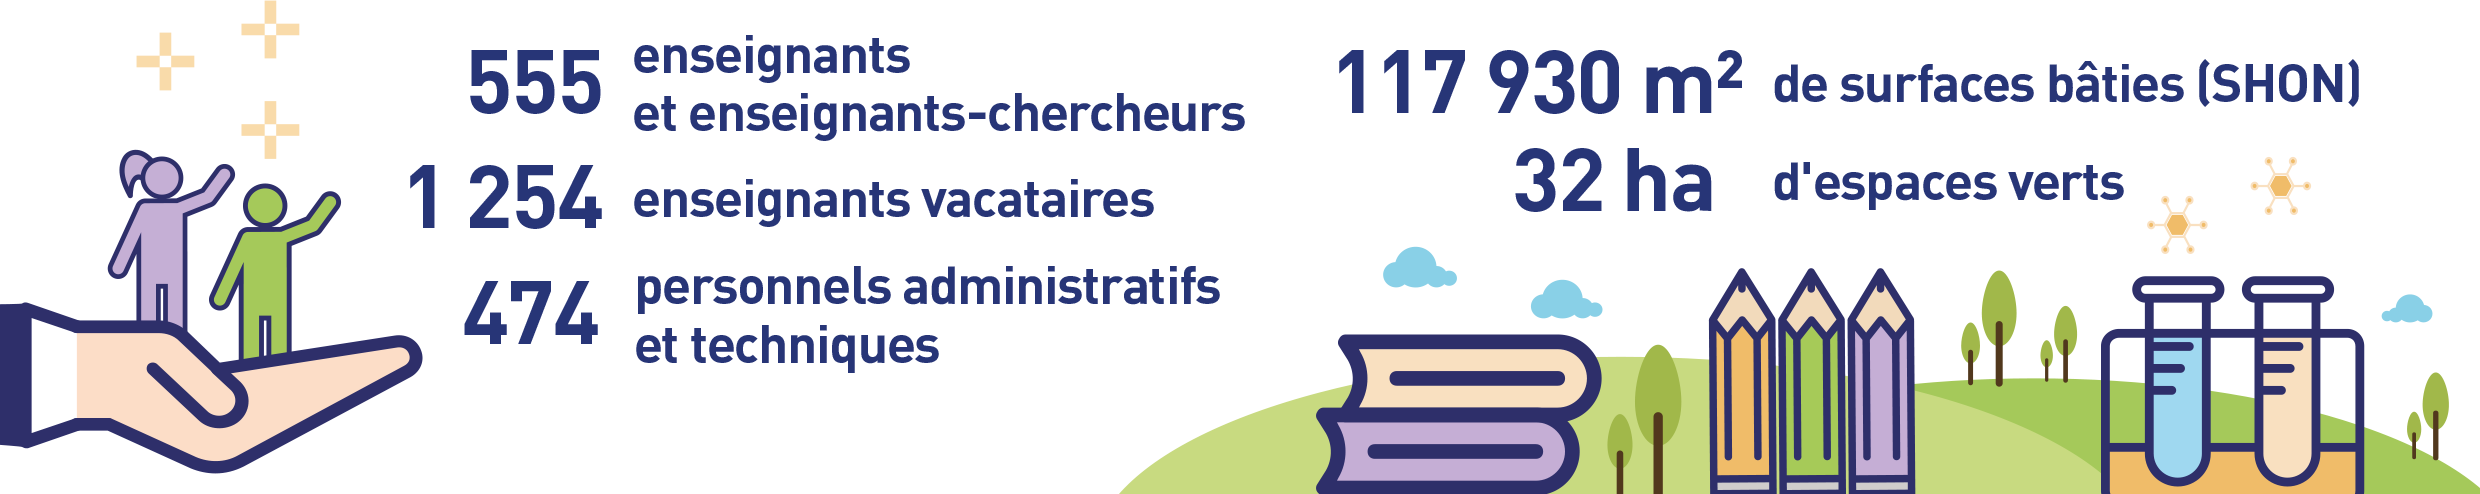
\includegraphics[width=\linewidth]{UHA_personnel_surface}
		\end{frame}
		\begin{frame}[t]
			\frametitle{L'Université de Haute Alsace: éducation}
			\centering
			\vspace{10pt}
			
\includegraphics[width=\linewidth]{UHA_etudiants}
			\\\vspace{30pt}
			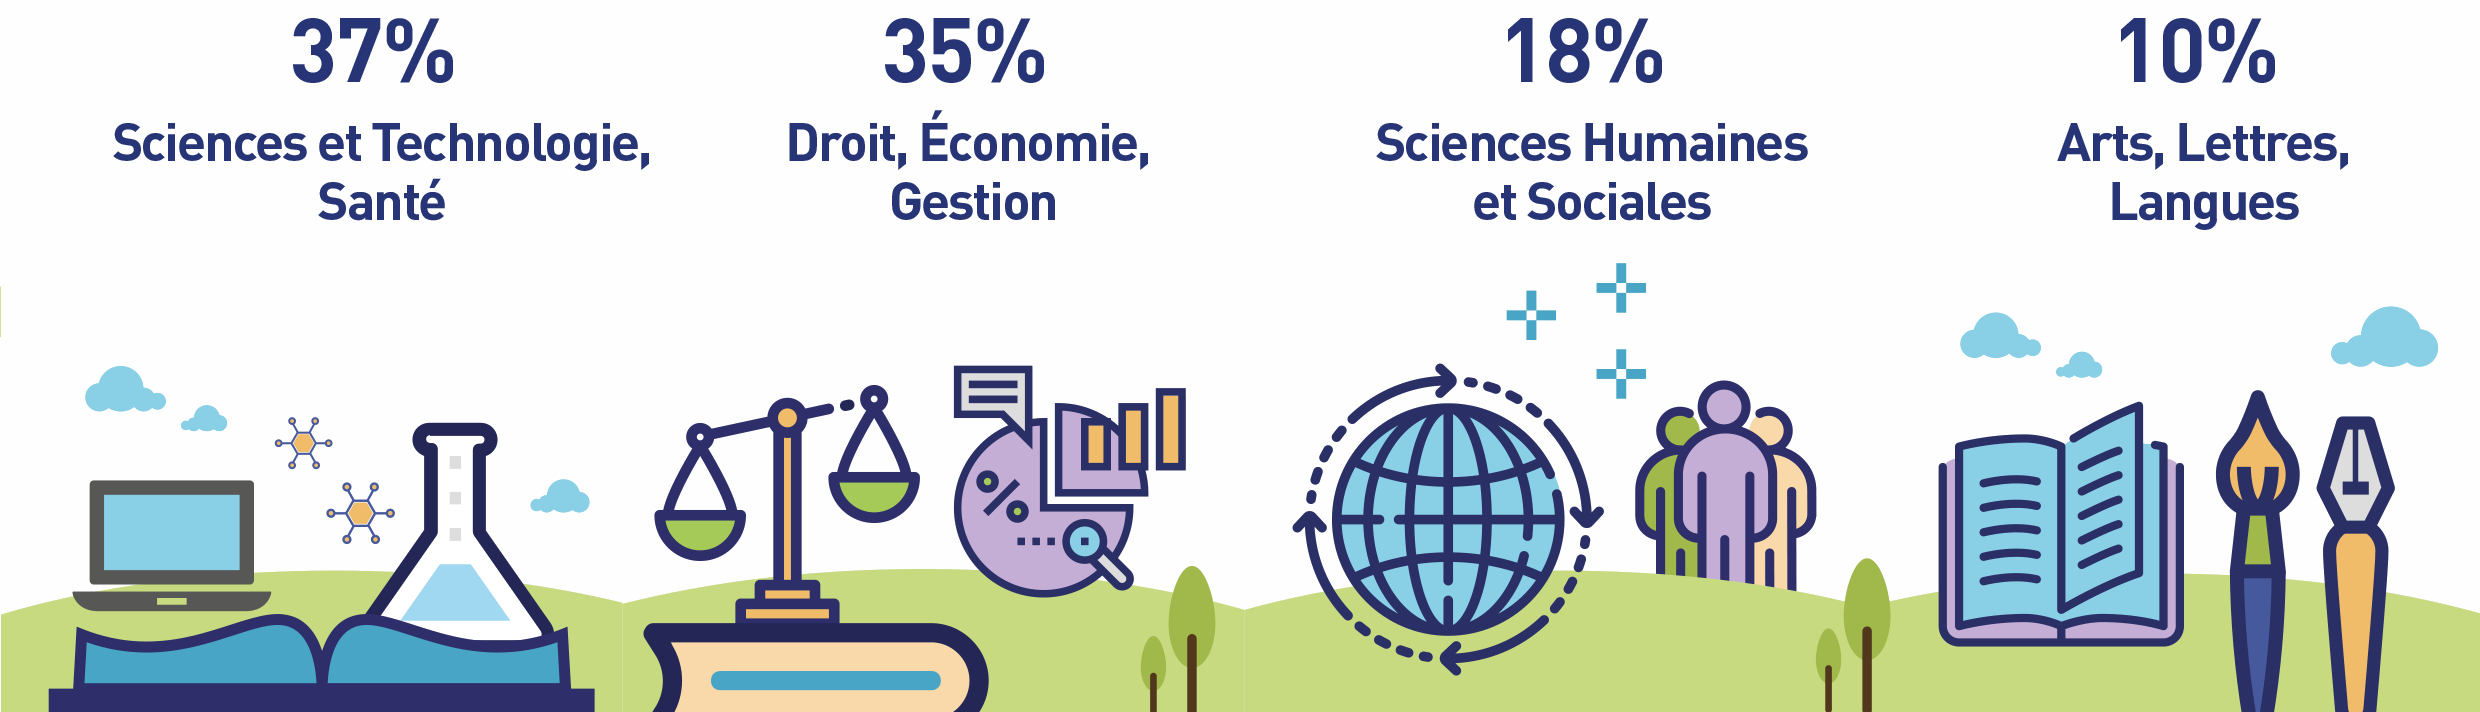
\includegraphics[width=\linewidth]{UHA_etudiants_repartition}
		\end{frame}
		\begin{frame}
			\frametitle{L'Université de Haute Alsace: recherche}
			\centering
			\vspace{10pt}
			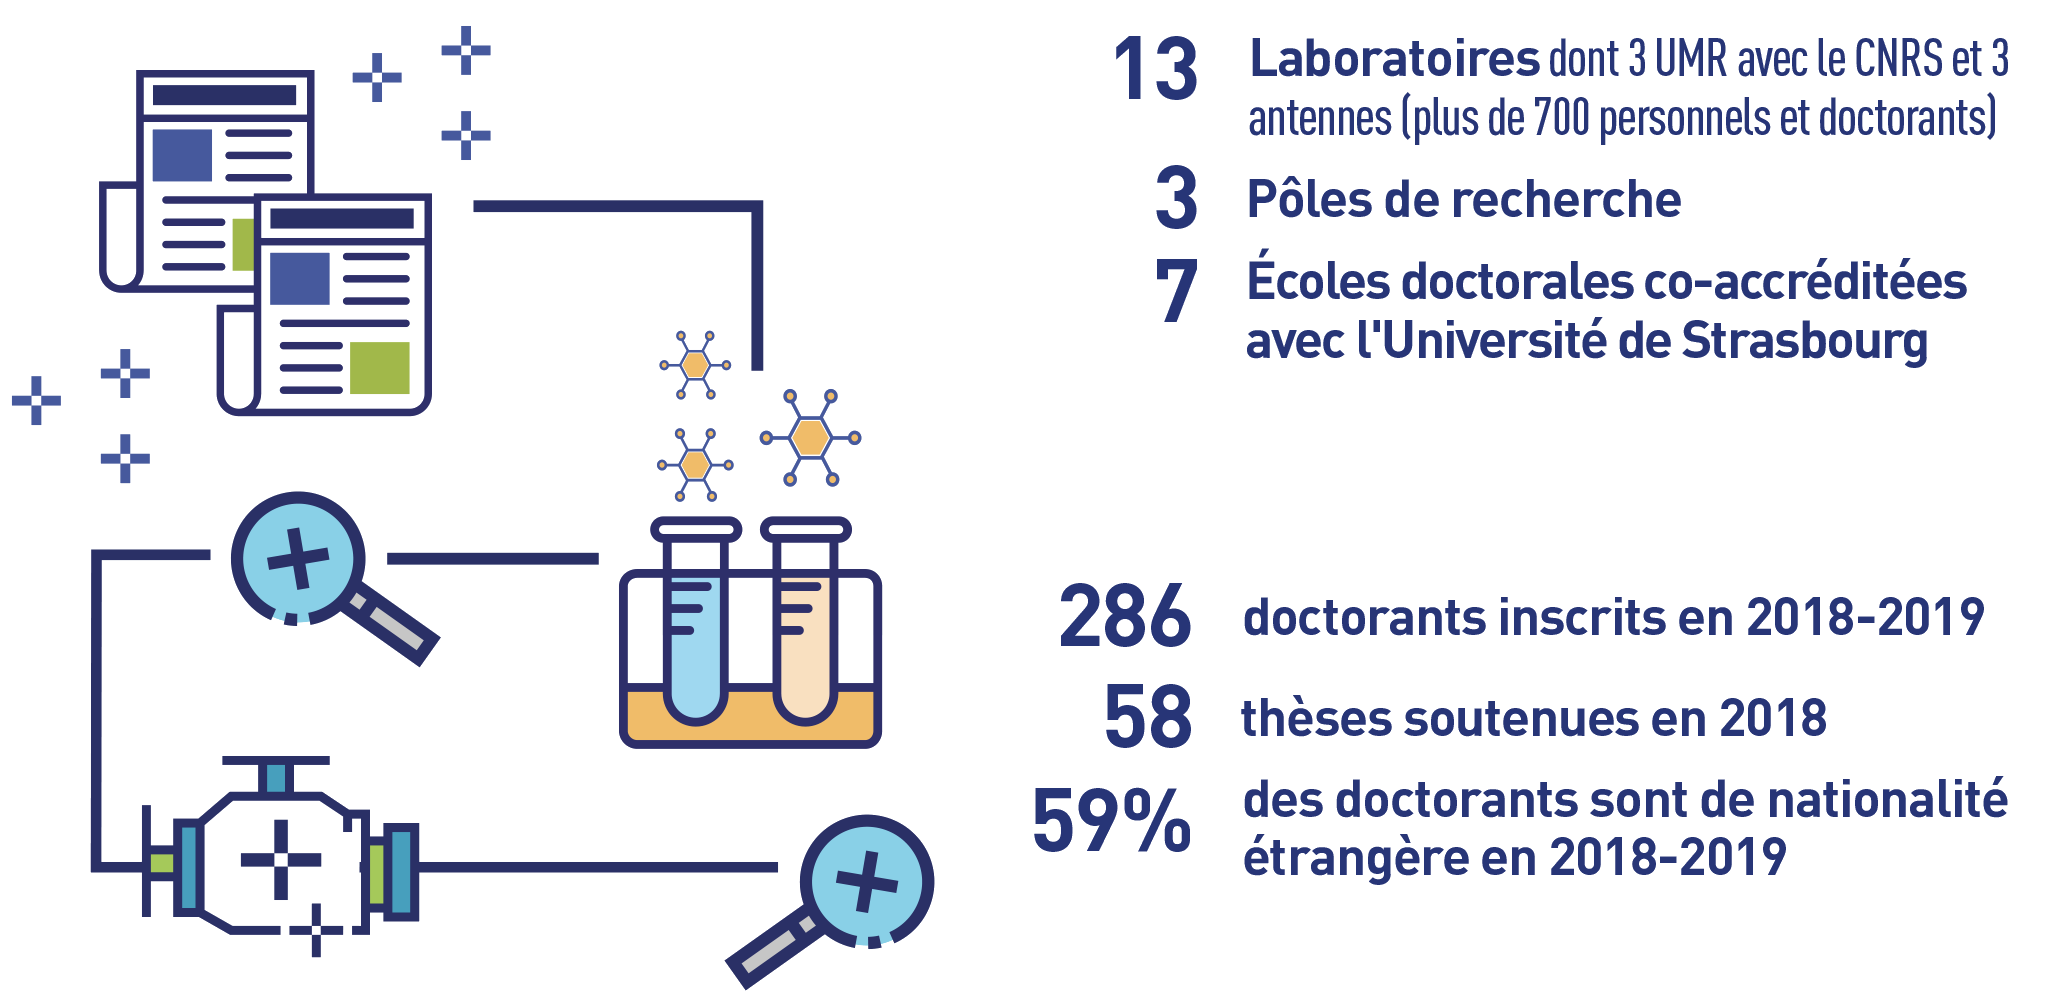
\includegraphics[width=\linewidth]{UHA_recherche}
		\end{frame}
		\begin{frame}[t]
			\frametitle{L'Université de Haute Alsace: laboratoires}
			\begin{block}{Laboratoires}
				\begin{itemize}
					\item Pôle Chimie, Physique, Matériaux et Environnement
						\begin{itemize}
							\item[\(\blacktriangleright\)] GRE, IPHC, S2M, LIMA, LPIM, LVBE
						\end{itemize}
					\item[\(\blacktriangleright\)] Pôle Sciences pour l'Ingénieur
						\begin{itemize}
							\item IRIMAS, LPMT
						\end{itemize}
					\item[\(\blacktriangleright\)] Pôle Sciences Humaines et Sociales
						\begin{itemize}
							\item ARCHIMEDE, BETA, CERDACC, CREGO, CRESAT, ILLE, LISEC, SAGE
						\end{itemize}
				\end{itemize}
			\end{block}
			\centering
			\vspace{7.5pt}
			
\includegraphics[width=\linewidth]{IRIMAS}
		\end{frame}
		\begin{frame}
			\frametitle{L'IRIMAS}
			\centering
			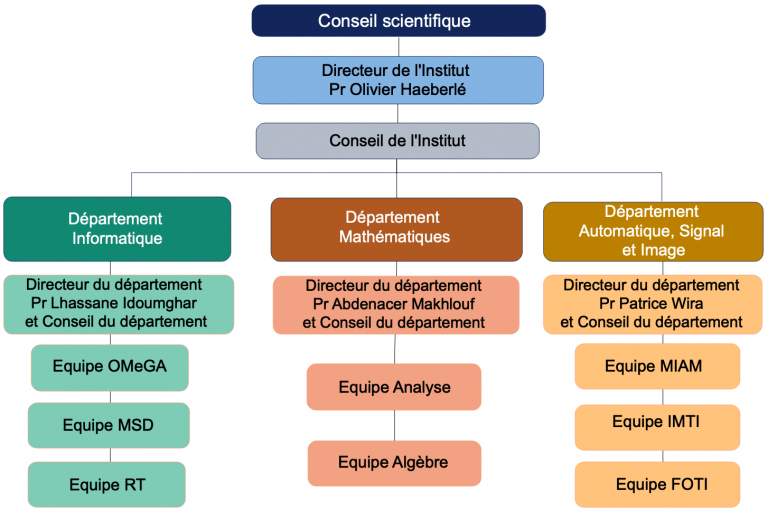
\includegraphics[width=0.9\linewidth]{irimas_organigramme}
		\end{frame}
	\section{Sujets du stage}
		\begin{frame}
			\frametitle{Définition du Unicost Set Cover Problem (USCP)}
			\begin{block}{Notation}
				\begin{itemize}
					\item \(U = \{u_1, u_2, u_3, \dots, u_m\}\), ensemble univers de \(m\) éléments
					\item \(S = \{s_1, s_2, \dots, s_n\}\), famille de \(n\) sous-ensembles de \(U\)
				\end{itemize}
			\end{block}
			\begin{block}<2->{Objectif}
				\begin{itemize}
					\item[\alert{\(\blacktriangleright\)}] Trouver une sous-famille de \(S\) la plus petite possible permettant de couvrir chaque élément de \(U\) au moins une fois.
					\item \(e\) est couvert par un sous-ensemble \(A\) si \(e \in A\).
				\end{itemize}
			\end{block}
		\end{frame}
		\begin{frame}
			\frametitle{Exemple minimal d'instance du USCP}
			\centering%
			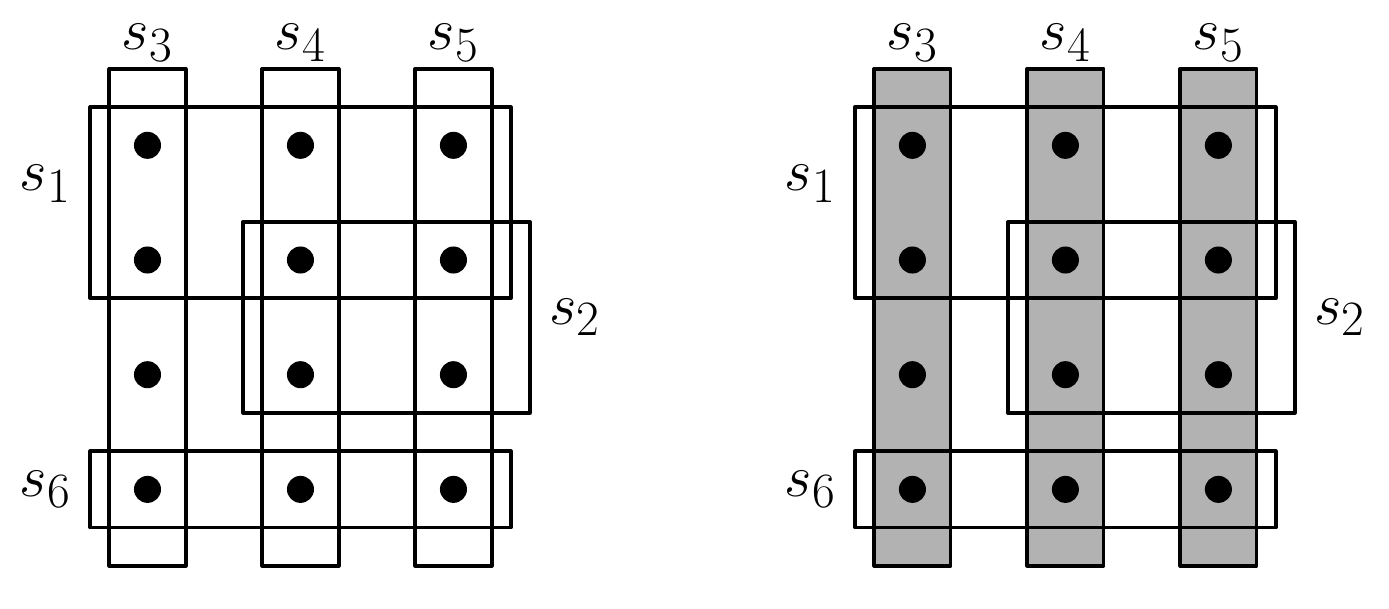
\includegraphics[width=0.85\linewidth]{uscp_example}%
		\end{frame}
		\begin{frame}
			\frametitle{Représentation du USCP}
			\[
			\begin{blockarray}{ccccccccc}
				& s_1 & s_2 & s_3 & s_4 & s_5 & s_6 & s_7 \\
				\begin{block}{c(ccccccc)c}
					    & 0 & 1 & 1 & 0 & 0 & 0 & 1 & u_1\\
					    & 0 & 0 & 1 & 0 & 1 & 1 & 0 & u_2\\
					A = & 1 & 1 & 0 & 1 & 0 & 1 & 0 & u_3\\
					    & 0 & 0 & 0 & 0 & 1 & 1 & 1 & u_3\\
					    & 1 & 0 & 1 & 0 & 0 & 0 & 1 & u_4\\
				\end{block}
				\\
				\begin{block}{c(ccccccc)c}
					x_1 = & 0 & 0 & 1 & 0 & 0 & 1 & 0 &\\
				\end{block}
				\\
				\begin{block}{c(ccccccc)c}
					x_2 = & 0 & 0 & 0 & 0 & 0 & 1 & 1 &\\
				\end{block}
			\end{blockarray}
			\]
		\end{frame}
		\begin{frame}
			\frametitle{Résolution}
			\begin{block}{Complexité}
				C'est l'un des 21 problèmes NP-complets de \citeauthor{Karp1972}.
			\end{block}
			\hfill\\
			\centering
			%\includegraphics[width=0.9\linewidth]{karp_reduction_tree}%
			\uncover<2->{%
				%\includegraphics[width=0.9\linewidth]{exhaustive_search_time}%
				\begin{block}{Méthode de résolution}
					\begin{itemize}
						\item[\(\blacktriangleright\)] Algorithme mémétique a 2 individus inspiré de Hybrid Evolutionary Algorithm in Duet (HEAD)
					\end{itemize}
				\end{block}
			}
		\end{frame}
	\section{Travail réalisé}
		\begin{frame}
			\frametitle{L'algorithme Row Weighting Local Search}
			\[
			\begin{blockarray}{cccccccccc}
				\uncover<3->{
					{\color{Corange}scores} & {\color{Corange}6} & {\color{Corange}-5} & {\color{Corange}6} & {\color{Corange}0} & {\color{Corange}0} & {\color{Corange}-9} & {\color{Corange}6} \\
					\\
				}
				& s_1 & s_2 & s_3 & s_4 & s_5 & s_6 & s_7 & & \uncover<2->{{\color{Cgreen}poids}} \\
				\begin{block}{c(ccccccc)cc}
					    & 0 & 1 & 1 & 0 & 0 & 0 & 1 & u_1 & \uncover<2->{{\color{Cgreen}5}}\\
					    & 0 & 0 & 1 & 0 & 1 & 1 & 0 & u_2 & \uncover<2->{{\color{Cgreen}7}}\\
					A = & 1 & 1 & 0 & 1 & 0 & 1 & 0 & u_3 & \uncover<2->{{\color{Cgreen}3}}\\
					    & 0 & 0 & 0 & 0 & 1 & 1 & 1 & u_3 & \uncover<2->{{\color{Cgreen}2}}\\
					    & 1 & 0 & 1 & 0 & 0 & 0 & 1 & u_4 & \uncover<2->{{\color{Cgreen}6}}\\
				\end{block}
				\\
				\begin{block}{c(ccccccc)cc}
					x = & 0 & 1 & 0 & 0 & 0 & 1 & 0 &\\
				\end{block}
			\end{blockarray}
			\]
		\end{frame}
		\begin{frame}
			\frametitle{Algorithme mémétique version 1}
			\centering%
			\resizebox{\textwidth}{!}{\import{../figures/}{memetic_algorithm_v1.tex}}%
		\end{frame}
		\begin{frame}
			\frametitle{Algorithme mémétique version 2}
			\centering%
			\resizebox{\textwidth}{!}{\import{../figures/}{memetic_algorithm_v2.tex}}%
		\end{frame}
		\begin{frame}
			\frametitle{Algorithme mémétique version 3: MASC}
			\centering%
			\resizebox{\textwidth}{!}{\import{../figures/}{memetic_algorithm_v3.tex}}%
		\end{frame}
		\begin{frame}
			\frametitle{Détails techniques}
			\begin{center}
				\begin{minipage}[b]{0.47\textwidth}
					\begin{block}{Implémentation}
						\Cpp{}17, $\sim$10\,000 lignes, 3 cibles
						\begin{itemize}
							\item 1 librairie
								\begin{itemize}
									\item[\(\blacktriangleright\)] common
								\end{itemize}
							\item 2 programmes:
								\begin{itemize}
									\item[\(\blacktriangleright\)] solver
									\item[\(\blacktriangleright\)] printer
								\end{itemize}
						\end{itemize}
					\end{block}
				\end{minipage}
				\hfill{}
				\resizebox{0.5\textwidth}{!}{\import{../figures/}{USCP_repository_files_stats_lines.tex}}%
			\end{center}
		\end{frame}
	\section{Résultats}
		\begin{frame}
			\frametitle{Benchmarks}
			\begin{block}{Machines}
				Cluster HPC du méso-centre de l'université de Strasbourg
			\end{block}
			\begin{block}{Instances}
				4.1, 4.2, 4.3, 4.4, 4.5, 4.6, 4.7, 4.8, 4.9, 4.10, 5.1, 5.2, 5.3, 5.4, 5.5, 5.6, 5.7, 5.8, 5.9, 5.10, 6.1, 6.2, 6.3, 6.4, 6.5, A.1, A.2, A.3, A.4, A.5, B.1, B.2, B.3, B.4, B.5, C.1, C.2, C.3, C.4, C.5, D.1, D.2, D.3, D.4, D.5, E.1, E.2, E.3, E.4, E.5, NRE.1, NRE.2, NRE.3, NRE.4, NRE.5, NRF.1, NRF.2, NRF.3, NRF.4, NRF.5, NRG.1, NRG.2, NRG.3, NRG.4, NRG.5, NRH.1, NRH.2, NRH.3, NRH.4, NRH.5, CLR10, CLR11, CLR12, CLR13, CYC6, CYC7, CYC8, CYC9, CYC10, CYC11, RAIL507, RAIL516, RAIL582, RAIL2536, RAIL2586, RAIL4284, RAIL4872, STS9, STS15, STS27, STS45, STS81, STS135, STS243, STS405, STS729, STS1215, STS2187
			\end{block}
		\end{frame}
		\begin{frame}
			\frametitle{Instances CYC: détails}
			\centering
			\begin{tabular}{ccccc}
				\toprule
				Instance & Lignes & Colonnes & Densité & Coûts\\
				\midrule
				CYC6 & 240 & 192 & 2.1\% & [1;1]\\
				CYC7 & 672 & 448 & 0.9\% & [1;1]\\
				CYC8 & 1\,792 & 1\,024 & 0.4\% & [1;1]\\
				CYC9 & 4\,608 & 2\,304 & 0.2\% & [1;1]\\
				CYC10 & 11\,520 & 5\,120 & 0.1\% & [1;1]\\
				CYC11 & 28\,160 & 11\,264 & 0.04\% & [1;1]\\
				\bottomrule
			\end{tabular}
		\end{frame}
		\begin{frame}
			\frametitle{Instances CYC: résultats}
			\scriptsize
			\begin{tabular}{lr{c}rrr{c}rrr}
				\toprule
				\multirow{2}{*}{\raisebox{-\heavyrulewidth}{Inst.}} & \multirow{2}{*}{\raisebox{-\heavyrulewidth}{BKS}} && \multicolumn{3}{l}{RWLS} && \multicolumn{3}{l}{MASC}\\
				\cmidrule{4-6}\cmidrule{8-10}
				 & && Best & \multicolumn{1}{c}{\#Best} & \multicolumn{1}{c}{Time(s)} && Best & \multicolumn{1}{c}{\#Best} & \multicolumn{1}{c}{Time(s)}\\
				\midrule
				CYC6 & 60  && \textbf{60} & 10 & 0.00 && \textbf{60} & 10 & 0.19 \\
				CYC7 & 144 && \textbf{144} & 10 & 0.02 && \textbf{144} & 10 & 0.33 \\
				CYC8 & 342 && \textbf{342} & 10 & 0.30 && \textbf{342} & 10 & 1.44 \\
				CYC9 & 772 && \textbf{772} & 2 & 266.70 && \textbf{772} & 6 & 103.95 \\
				CYC10 & 1\,798 && \textbf{1\,798} & 7 & 663.73 && \textbf{1\,792*} & 8 & 267.99 \\
				CYC11 & 3\,968 && \textbf{3\,968} & 1 & 520.69 && \textbf{3\,968} & 1 & 275.82 \\
			\end{tabular}
		\end{frame}
	\section{Conclusion}
		\begin{frame}
			\frametitle{Soumissions à 2 conférences}
			\begin{block}{ROADEF2020}
				21\textsuperscript{ème} congrès de la Société française de recherche opérationnelle et d'aide à la décision
				\begin{itemize}
					\item[\(\blacktriangleright\)] accepté le 21/12/2019
				\end{itemize}
			\end{block}
			\vspace{20pt}
			\begin{block}{LION14}
				14\textsuperscript{th} Learning and Intelligent OptimizatioN Conference
				\begin{itemize}
					\item[\(\blacktriangleright\)] accepté le 18/02/2020
				\end{itemize}
			\end{block}
		\end{frame}
		\begin{frame}[plain]
			\utbmclosingframe{Merci de votre attention}
		\end{frame}
	\appendix
	\section*{Références}
		\begin{frame}[t,allowframebreaks]
			\frametitle{Références}
			\printbibliography[heading=none]{}
		\end{frame}
	\section*{Informations supplémentaires}
		\begin{frame}
			\frametitle{Planning}
			\resizebox{0.85\paperwidth}{!}{\import{../figures/}{planning.tex}}%
		\end{frame}
		\begin{frame}
			\frametitle{Fonctionnement de RWLS}
			Étapes de Row Weighting Local Search (RWLS):
			\begin{enumerate}%[label=(\arabic*)]
				\item\tikzremember{RWLS1}tant que la solution est valide:
					\begin{enumerate}%[label=(\alph*)]
						\item\tikzremember{RWLS1a}enregistrer la solution comme la meilleure rencontrée jusqu'à présent
						\item\tikzremember{RWLS1b}\textbf{retirer} le sous-ensemble avec le meilleur score de la solution
					\end{enumerate}
				\item\tikzremember{RWLS2}\textbf{retirer} le sous-ensemble avec le meilleur score de la solution
				\item\tikzremember{RWLS3}sélectionner aléatoirement un élément non-couvert
				\item\tikzremember{RWLS4}\textbf{ajouter} le sous-ensemble avec le meilleur score couvrant cet élément (les stratégies tabou empêchant de boucler)
				\item\tikzremember{RWLS5}rendre le sous ensemble ajouté tabou et incrémenter le nombre d'étapes
			\end{enumerate}
			\begin{tikzpicture}[remember picture,overlay,x=1pt,y=1pt]
				\draw[->,>=Latex,dashed] ($(RWLS5)+(-15,0)$) -- ++(-12.5,0) |- ($(RWLS1)+(-15,0)$);
				\draw[->,>=Latex,dashed] ($(RWLS1b)+(-15,0)$) -| ($(RWLS1)+(-10,-7.5)$);
			\end{tikzpicture}
		\end{frame}
		\begin{frame}
			\frametitle{OR-Library: instances aléatoires}
			\centering
			\begin{tabular}{cccccc}
	\toprule
	Ensemble & Nb. instances & Lignes & Colonnes & Densité & Coûts\\
	\midrule
	4 & 10 & 200 & 1\,000 & 2\% & [1;100] \\
	5 & 10 & 200 & 2\,000 & 2\% & [1;100] \\
	6 & 5 & 200 & 1\,000 & 5\% & [1;100] \\
	A & 5 & 300 & 3\,000 & 2\% & [1;100] \\
	B & 5 & 300 & 3\,000 & 5\% & [1;100] \\
	C & 5 & 400 & 4\,000 & 2\% & [1;100] \\
	D & 5 & 400 & 4\,000 & 5\% & [1;100] \\
	E & 5 & 50 & 500 & 20\% & [1;1] \\
	NRE & 5 & 500 & 5\,000 & 10\% & [1;100] \\
	NRF & 5 & 500 & 5\,000 & 20\% & [1;100] \\
	NRG & 5 & 1\,000 & 10\,000 & 2\% & [1;100] \\
	NRH & 5 & 1\,000 & 10\,000 & 5\% & [1;100] \\
	\bottomrule
\end{tabular}

		\end{frame}
		\begin{frame}
			\frametitle{OR-Library: instances CYC CLR}
			\centering
			\begin{tabular}{ccccc}
	\toprule
	Instance & Lignes & Colonnes & Densité & Coûts\\
	\midrule
	CYC6 & 240 & 192 & 2.1\% & [1;1]\\
	CYC7 & 672 & 448 & 0.9\% & [1;1]\\
	CYC8 & 1\,792 & 1\,024 & 0.4\% & [1;1]\\
	CYC9 & 4\,608 & 2\,304 & 0.2\% & [1;1]\\
	CYC10 & 11\,520 & 5\,120 & 0.1\% & [1;1]\\
	CYC11 & 28\,160 & 11\,264 & 0.04\% & [1;1]\\
	CLR10 & 511 & 210 & 12\% & [1;1]\\
	CLR11 & 1\,023 & 330 & 12\% & [1;1]\\
	CLR12 & 2\,047 & 495 & 12\% & [1;1]\\
	CLR13 & 4\,095 & 715 & 12\% & [1;1]\\
	\bottomrule
\end{tabular}

		\end{frame}
		\begin{frame}
			\frametitle{OR-Library: instances RAIL}
			\centering
			\begin{tabular}{ccccc}
	\toprule
	Instance & Lignes & Colonnes & Densité & Coûts\\
	\midrule
	RAIL507 & 507 & 63\,009 & 1.3\% & [1;2]\\
	RAIL516 & 516 & 47\,311 & 1.3\% & [1;2]\\
	RAIL582 & 582 & 55\,515 & 1.2\% & [1;2]\\
	RAIL2536 & 2\,536 & 1\,081\,841 & 0.4\% & [1;2]\\
	RAIL2586 & 2\,586 & 920\,683 & 0.3\% & [1;2]\\
	RAIL4284 & 4\,284 & 1\,092\,610 & 0.2\% & [1;2]\\
	RAIL4872 & 4\,872 & 968\,672 & 0.2\% & [1;2]\\
	\bottomrule
\end{tabular}

		\end{frame}
		\begin{frame}
			\frametitle{Instances issues des STS}
			\centering
			\begin{tabular}{ccccc}
	\toprule
	Instance & Lignes & Colonnes & Densité & Coûts\\
	\midrule
	STS9 & 12 & 9 & 33.3\% & [1;1]\\
	STS15 & 35 & 15 & 20\% & [1;1]\\
	STS27 & 117 & 27 & 11.1\% & [1;1]\\
	STS45 & 330 & 45 & 6.7\% & [1;1]\\
	STS81 & 1\,080 & 81 & 3.7\% & [1;1]\\
	STS135 & 3\,015 & 135 & 2.2\% & [1;1]\\
	STS243 & 9\,801 & 243 & 1.2\% & [1;1]\\
	STS405 & 27\,270 & 405 & 0.7\% & [1;1]\\
	STS729 & 88\,452 & 729 & 0.4\% & [1;1]\\
	STS1215 & 245\,835 & 1\,215 & 0.2\% & [1;1]\\
	STS2187 & 796\,797 & 2\,187 & 0.1\% & [1;1]\\
	\bottomrule
\end{tabular}

		\end{frame}
		\begin{frame}
			\frametitle{Réduction appliquée aux instances RAIL}
			\centering
			\begin{tabular}{lrrrrr}
	\toprule
	Instance & Lignes & Colonnes & \makecell{Colonnes\\inclues} & \makecell{Lignes\\couvertes} & \makecell{Colonnes\\dominées}\\
	\midrule
	RAIL507 & 507 & 63\,009 & 8 & 20 & 37\,842\\
	RAIL516 & 516 & 47\,311 & 27 & 62 & 8\,990\\
	RAIL582 & 582 & 55\,515 & 7 & 17 & 28\,311\\
	RAIL2536 & 2\,536 & 1\,081\,841 & 5 & 32 & 290\,967\\
	RAIL2586 & 2\,586 & 920\,683 & 50 & 155 & 496\,329\\
	RAIL4284 & 4\,284 & 1\,092\,610 & 17 & 76 & 436\,693\\
	RAIL4872 & 4\,872 & 968\,672 & 86 & 321 & 499\,406\\
	\bottomrule
\end{tabular}

		\end{frame}
		\begin{frame}
			\frametitle{USCP: Représentation binaire}%
			\resizebox{\textwidth}{!}{\includestandalone{../figures/binary_representation_solution_check}}%
		\end{frame}
		\begin{frame}
			\frametitle{Opérateurs de croisement implémentés}
			\begin{block}{Crossovers}
				identity, merge, greedy\_merge, subproblem\_random, subproblem\_greedy, extended\_subproblem\_random, extended\_subproblem\_greedy, subproblem\_rwls, extended\_subproblem\_rwls
			\end{block}
			\begin{block}{WCrossovers}
				reset, keep, average, mix\_random, add, difference, max, min, minmax, shuffle
			\end{block}
		\end{frame}
		\begin{frame}
			\frametitle{Commits par semaine}%
			\resizebox{\textwidth}{!}{\import{../figures/}{git_commits.tex}}%
		\end{frame}
		\begin{frame}
			\frametitle{Répartition du code}%
			\resizebox{\textwidth}{!}{\import{../figures/}{USCP_repository_files_stats.tex}}%
		\end{frame}
		\begin{frame}
			\frametitle{Utilisation du cluster HPC}%
			\resizebox{\textwidth}{!}{\import{../figures/}{hpc_usage.tex}}%
		\end{frame}
\end{document}
